\documentclass[letterpaper,12pt,preprint]{aastex}

% packages
\usepackage{amssymb,amsmath}

\begin{document}

\title{Spitzer Sgr target selection}
\author{Adrian M. Price-Whelan}

In this document, I'll explain how we selecting RR Lyrae (RRL) targets associated with the Sagittarius stream for Spitzer observation. Because the stream extends out beyond 60~kpc, many of these targets are quite expensive in terms of required Spitzer integration time. We've decided to only select RRLs that match the stream in both distance and radial velocity (at a given phase along the orbit), as compared to the Law \& Majewski 2010 simulation of the stream. The Catalina Sky Survey (CSS) recently published a catalog of $\sim$12,000 type-ab RRL stars identified from time-domain photometry, along with $\sim$1500 radial velocities. We use this catalog as our sample.

As an initial cut, we use the Sgr coordinate system from Majewski et al. (2003) to select all CSS RRLs within 20~kpc of the $B=0$ plane, and a Galactocentric distance $D_{\rm gc} > 15~{\rm kpc}$ (the inner halo is a mess). Figure~\ref{fig:css_all} shows (in Galactocentric cartesian coordinates) a) the distribution of all CSS RRLs, b) all RRLs that match the above cut, and c) the LM10 particles in the same coordinates. The leading arm is distinctly visible in the northern CSS data, and hints of the trailing arm are seen in the south. Note that there appears to be some offset between the CSS leading arm and the simulation --- this could be physical, but could also be an error in their distance calibration. I've also included a figure (Fig.~\ref{fig:css_vgsr}) that shows the radial velocities against Sgr longitude ($\Lambda$) for LM10 particles (grey) and the CSS RRLs (red), but no clear overdensities are visible.

Next we take 30 bins in $\Lambda$ and compute the median and $\pm$3-$\sigma$ distances for each bin from the LM10 particle data for the leading and trailing arm separately. We then find any star that could feasibly be within $\pm$3-$\sigma$ of the median distance to each arm, taking into account the distance errors. Figure~\ref{fig:lm10_selection} shows these (soft) margins overlaid with the LM10 particles, while figure~\ref{fig:css_selection} shows the CSS RRLs with RVs selected with this method. We ignore trailing arm data with $\Lambda>180$ since Belokurov et al. 2013 show with BHB stars that the trailing arm may not match the LM10 model past apocenter.

We then do the same thing with $v_{\rm gsr}$ by taking 30 bins in $\Lambda$ and repeating the above algorithm. Figure~\ref{fig:lm10_vgsr} shows the median and $\pm$3-$\sigma$ velocities for these bins, and figure~\ref{fig:css_vgsr} shows the CSS RRLs selected with this window. The remaining sample consists of 193 RR Lyrae, with a total required integration time of $\sim$1000 hr --- way over the budgeted time. We 1) want to get precise distances along many phases of the stream and 2) don't want to spend all of our time on distant targets which require the most exposure time. To select a subset, we take 5 stars at random from 15 degree bins in $\Lambda$. The final sample is shown in red in Figure~\ref{fig:final_sample}, with the other likely stream members in black, overplotted on the LM10 particles. 

\begin{figure}
\begin{center}
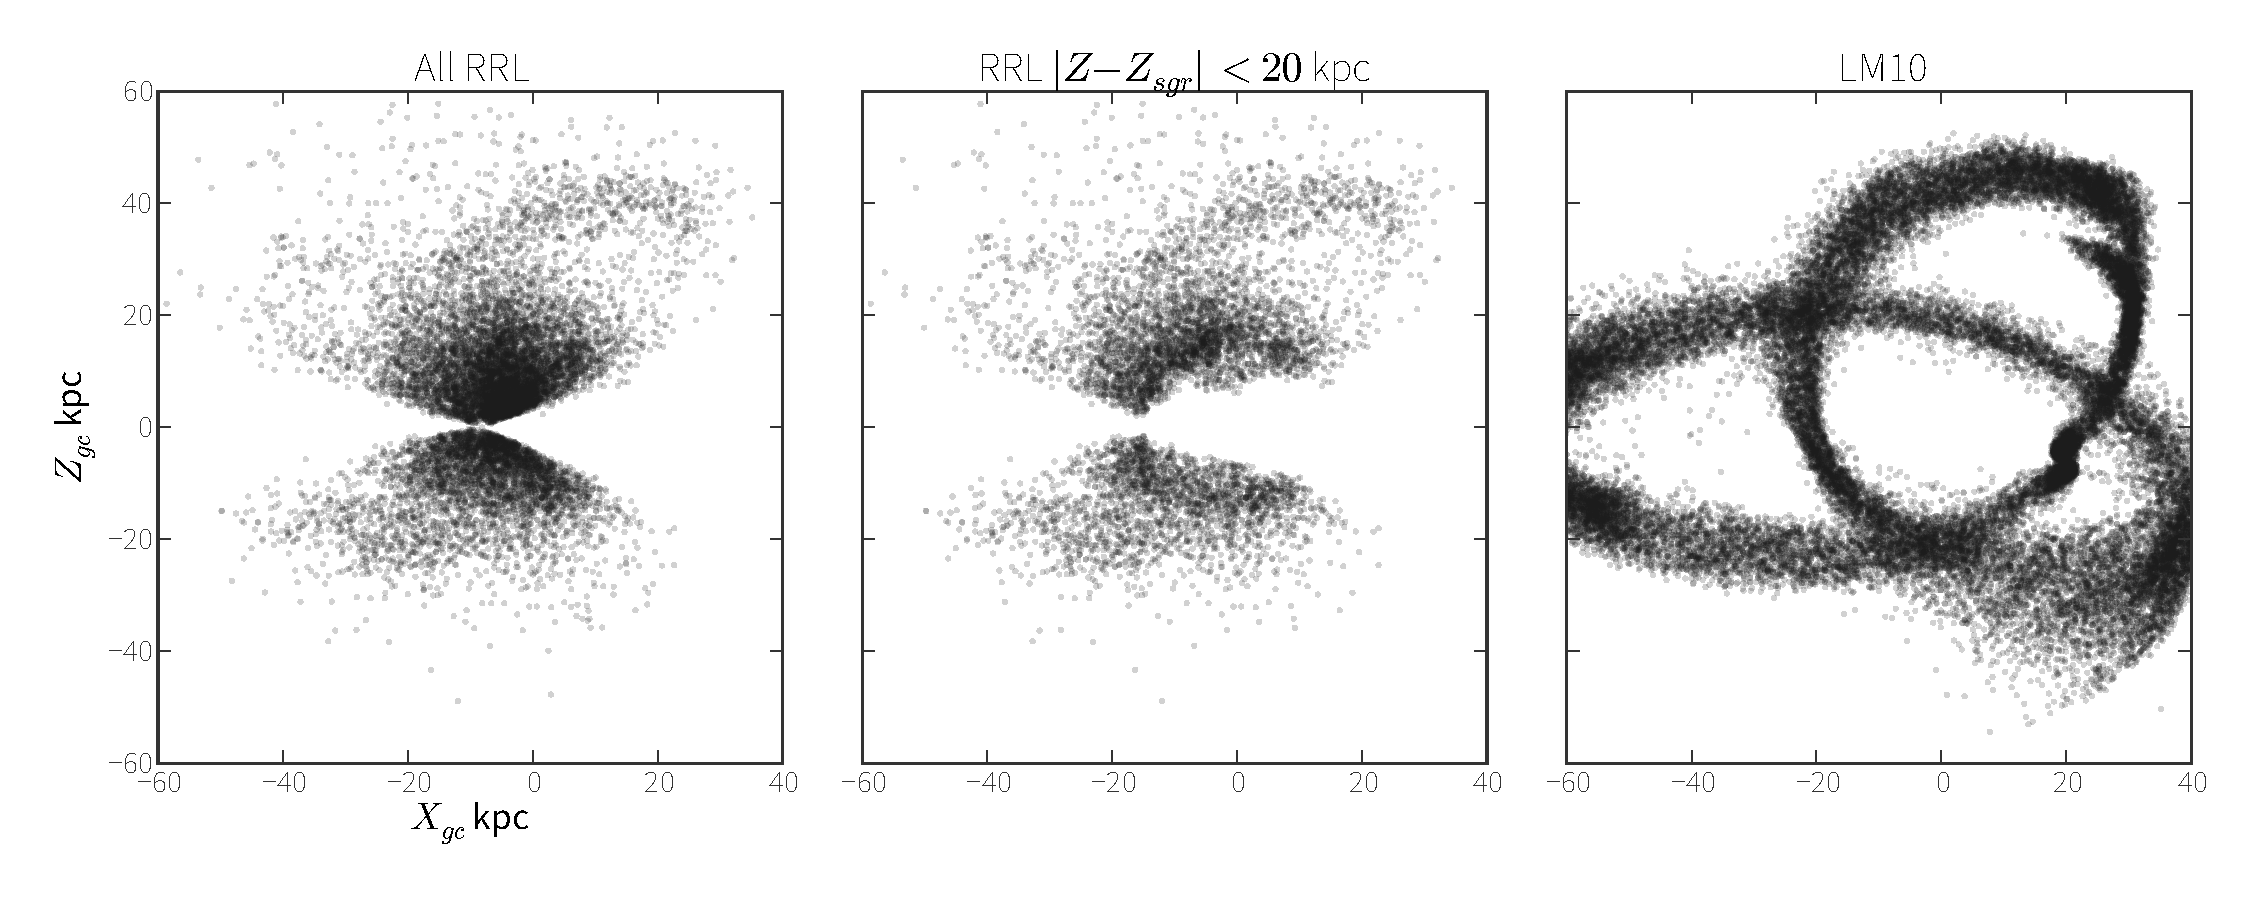
\includegraphics[width=0.9\textwidth]{catalina_all.pdf}
\caption{ From left to right: a) All CSS RRLs, b) CSS RRLs $<$ 20 kpc from the midplane of the Sgr coordinate system, and c) LM10 simulation particles. }\label{fig:css_all}
\end{center}
\end{figure}

\begin{figure}
\begin{center}
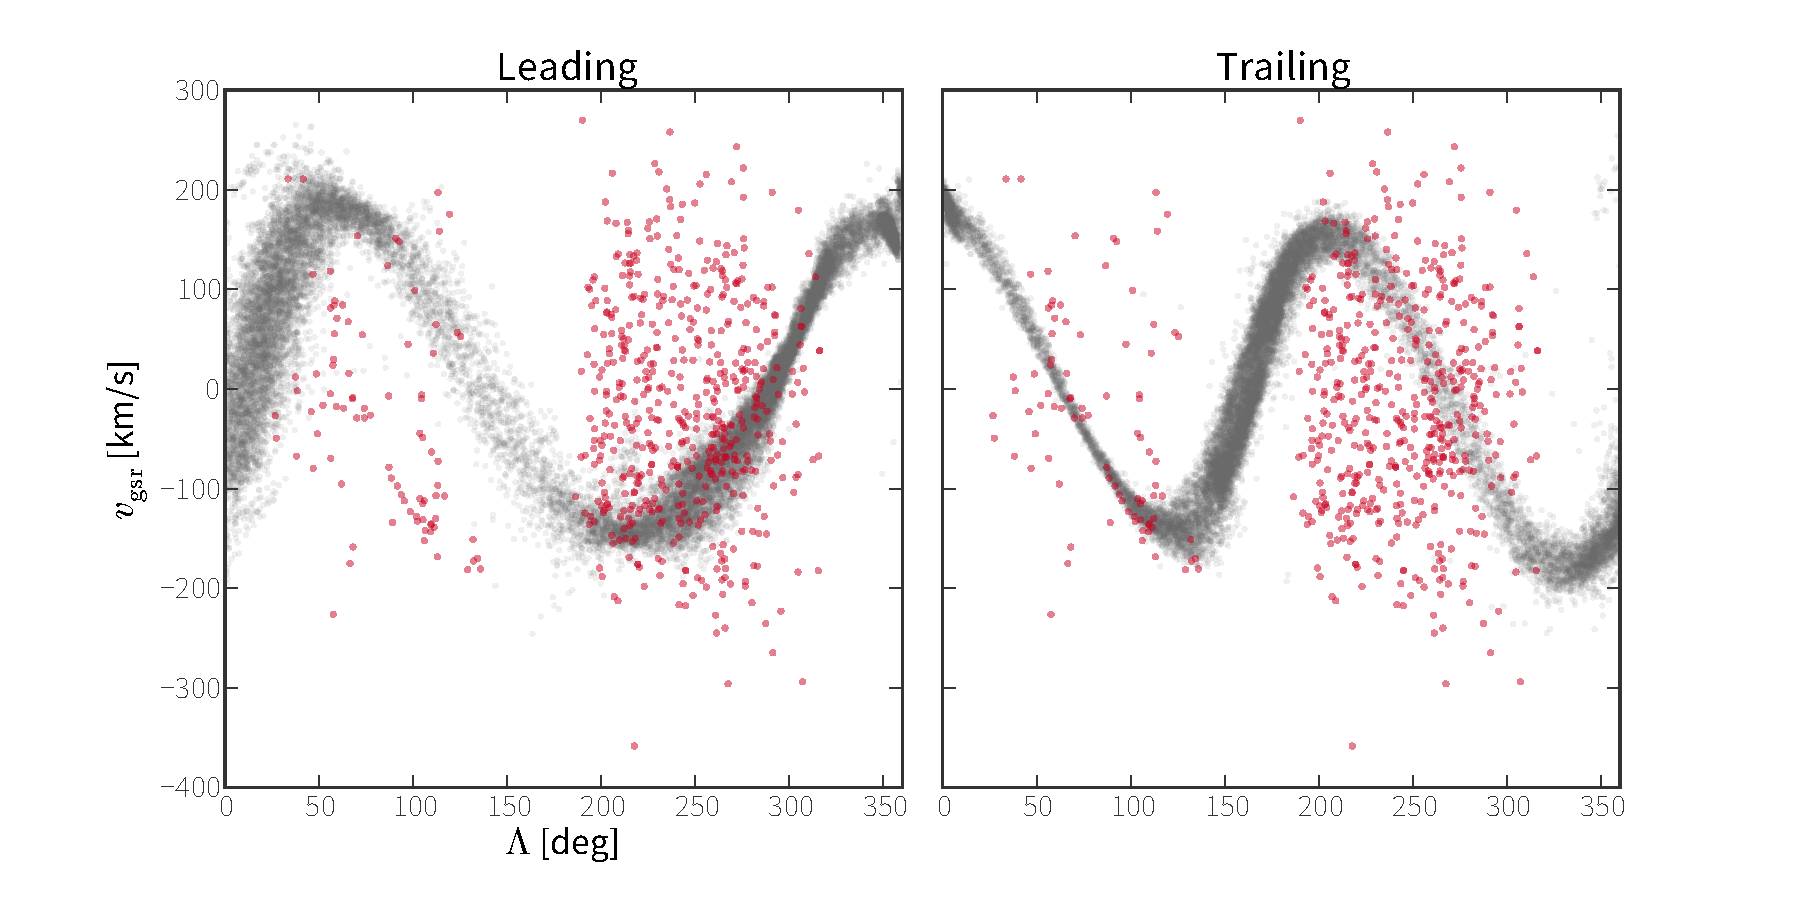
\includegraphics[width=0.75\textwidth]{catalina_all_vgsr.pdf}
\caption{ Galactocentric radial velocity for LM10 particles (grey) and CSS RRLs (red) for both the leading (left) and trailing (right) arms of Sgr debris. }\label{fig:css_vgsr}
\end{center}
\end{figure}

\begin{figure}
\begin{center}
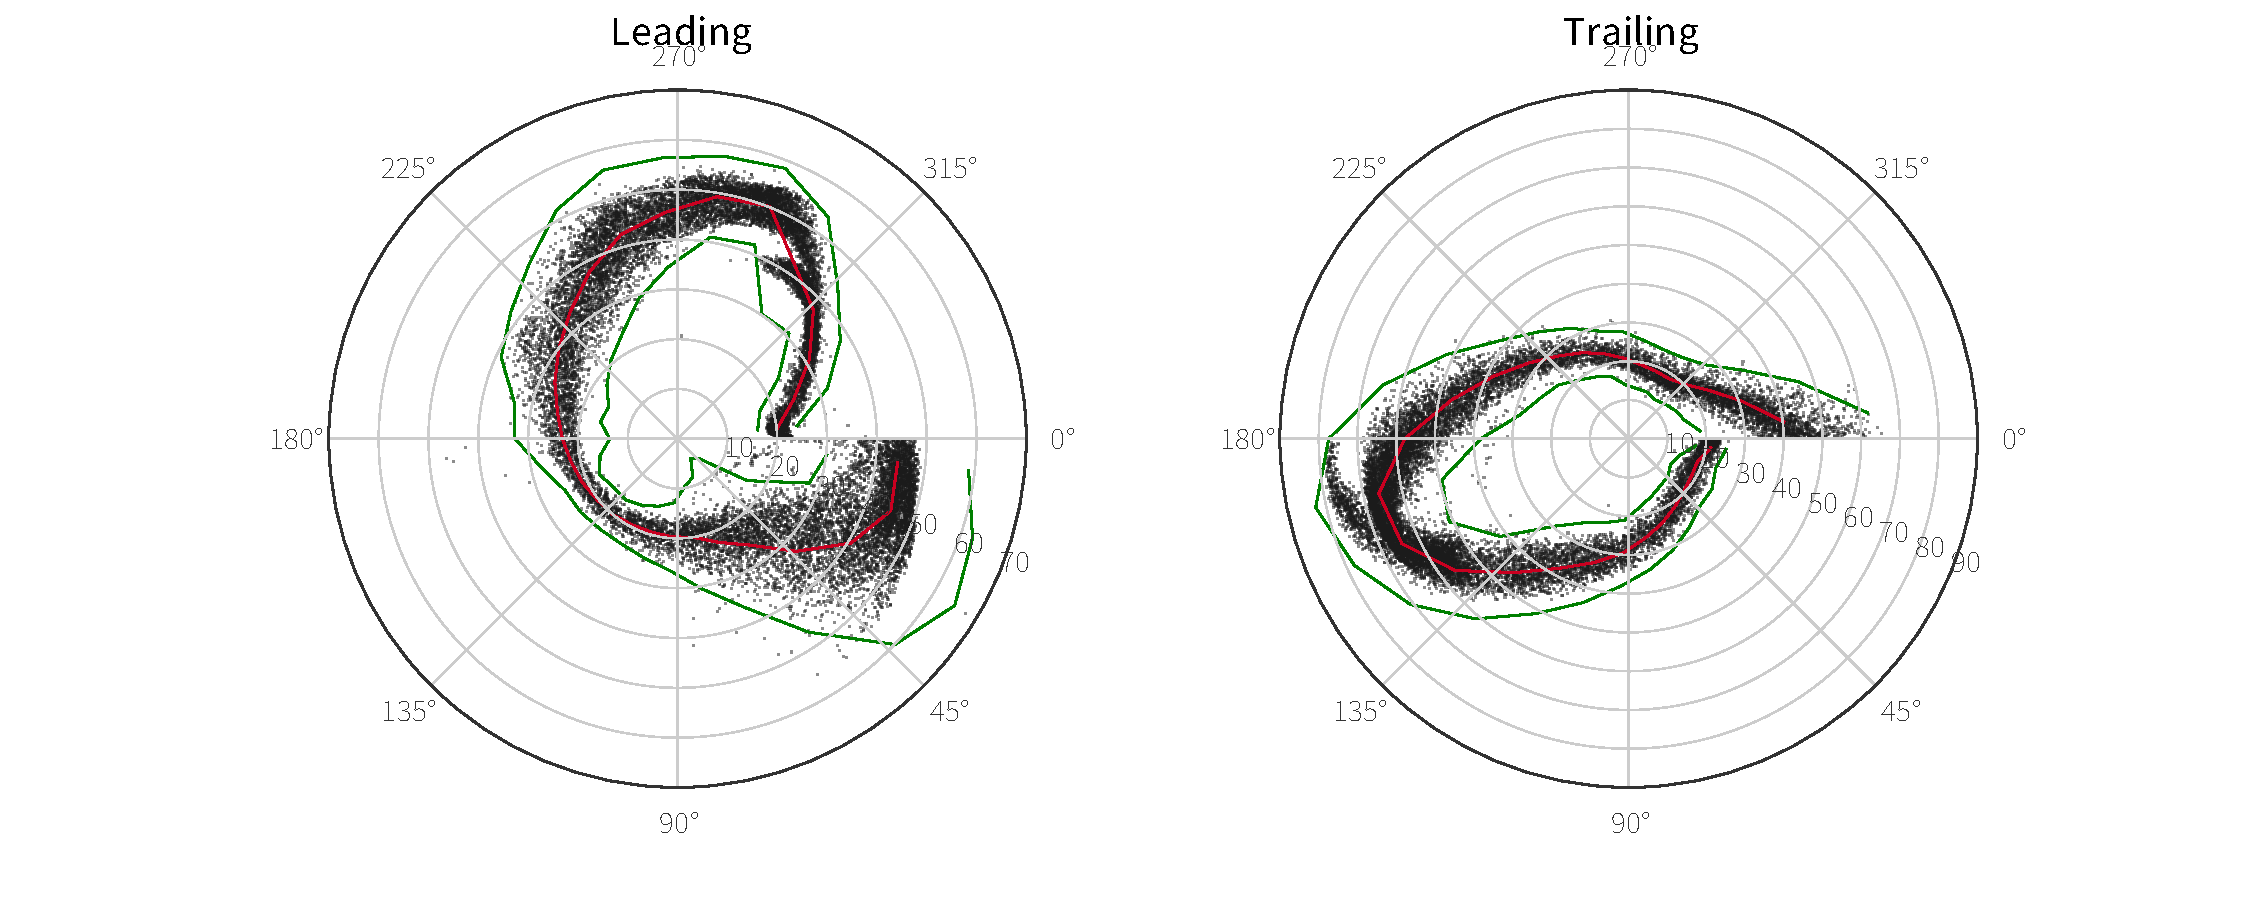
\includegraphics[width=\textwidth]{lm10_selection.pdf}
\caption{ LM10 particles from each Sgr arm, with median distance (red) and $\pm$3-$\sigma$ (green) distance values for 30 bins in $\Lambda$. }\label{fig:lm10_selection}
\end{center}
\end{figure}

\begin{figure}
\begin{center}
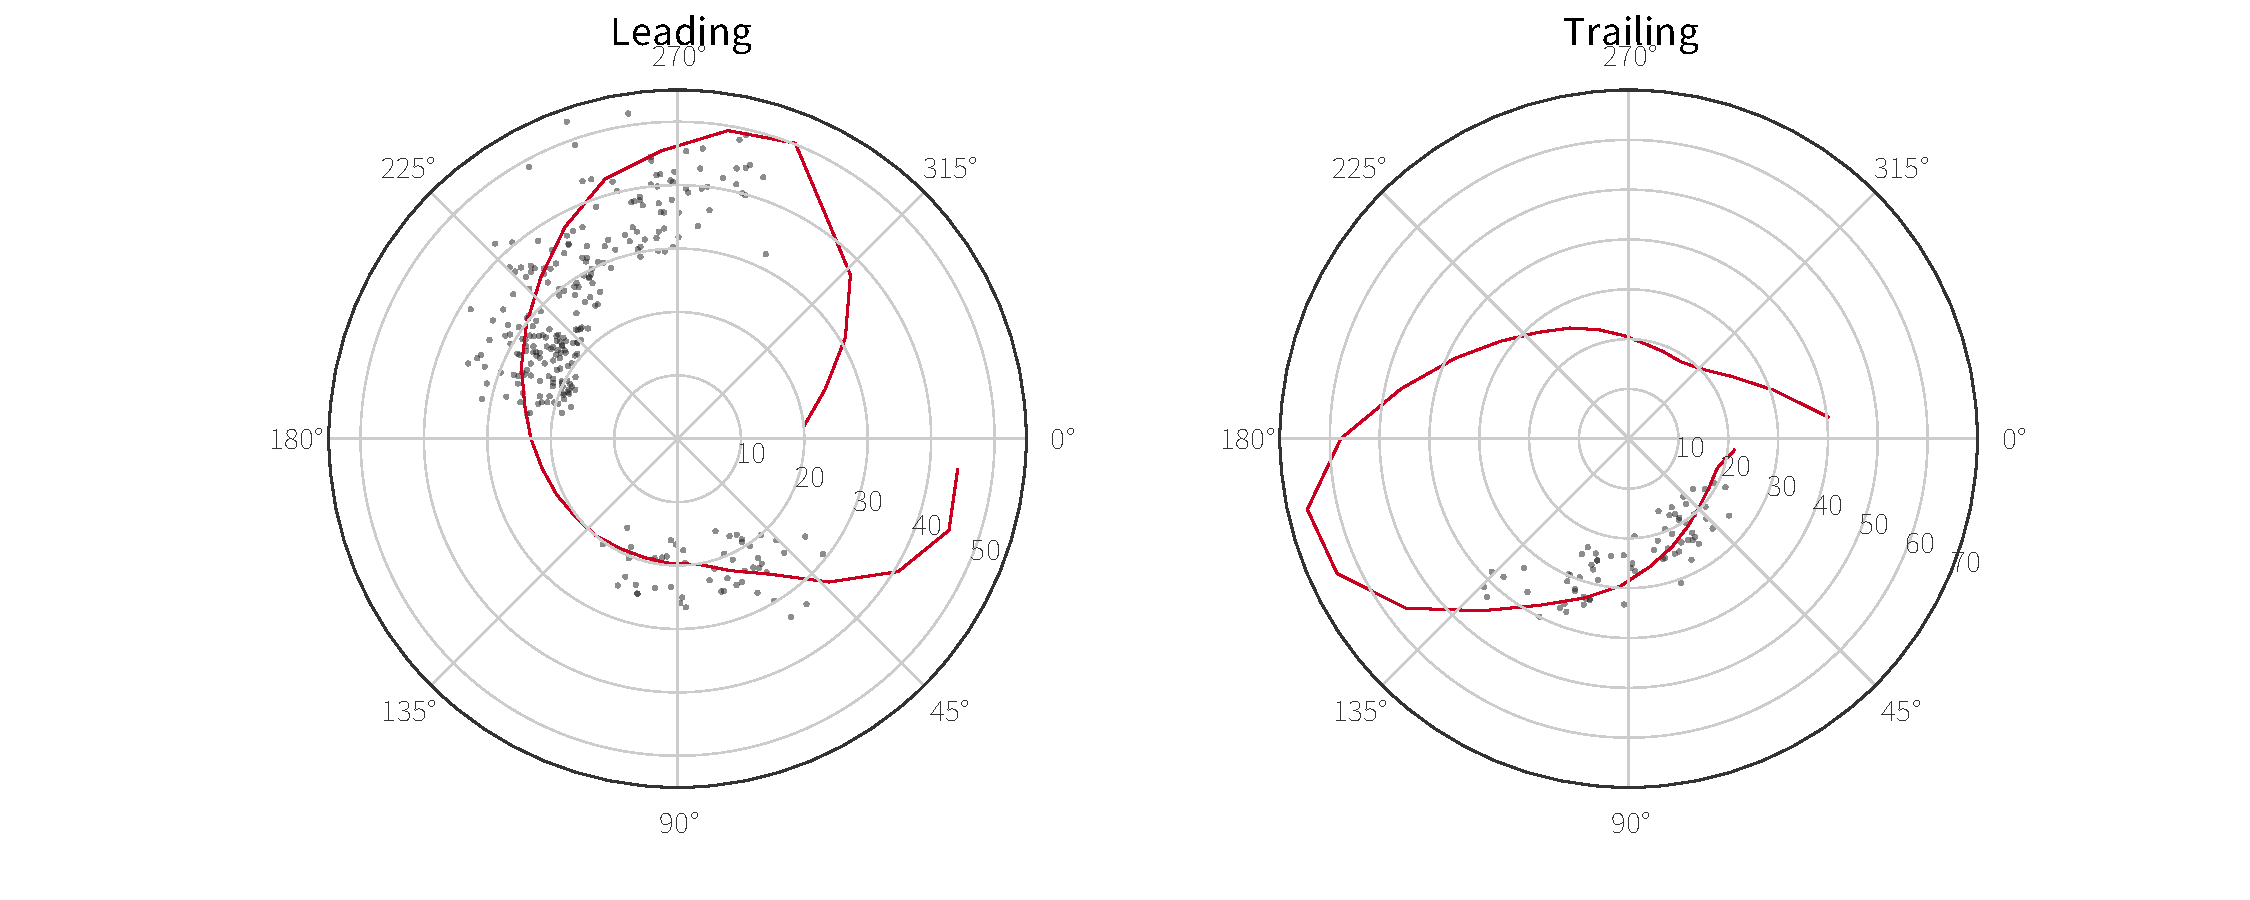
\includegraphics[width=\textwidth]{css_selection_vgsr.pdf}
\caption{ CSS RRLs with measured radial velocities selected to be within $\pm$3-$\sigma$ + distance error from the median LM10 distance in each bin from fig.~\ref{fig:lm10_selection}. }\label{fig:css_selection}
\end{center}
\end{figure}

\begin{figure}
\begin{center}
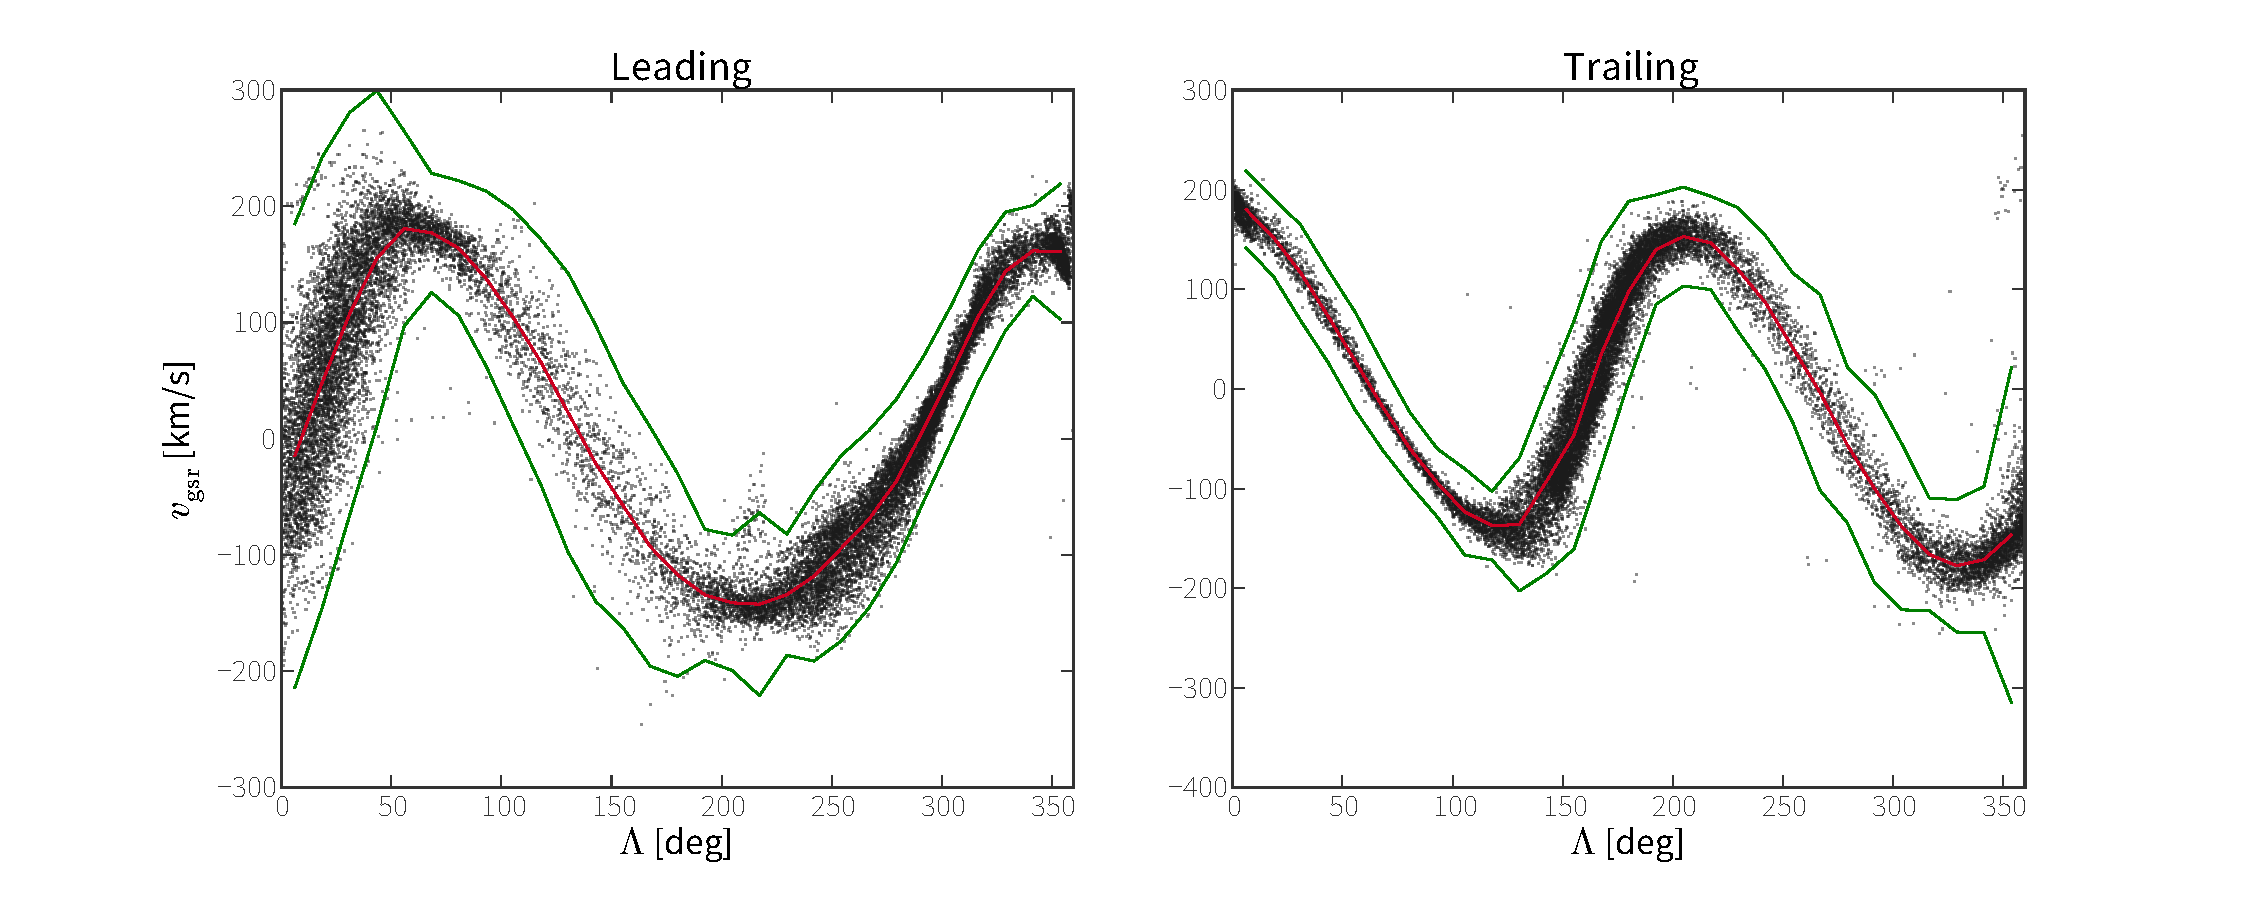
\includegraphics[width=\textwidth]{lm10_vgsr_selection.pdf}
\caption{ LM10 particles from each Sgr arm, with median radial velocity (red) and $\pm$3-$\sigma$ (green) values for 30 bins in $\Lambda$. }\label{fig:lm10_vgsr}
\end{center}
\end{figure}

\begin{figure}
\begin{center}
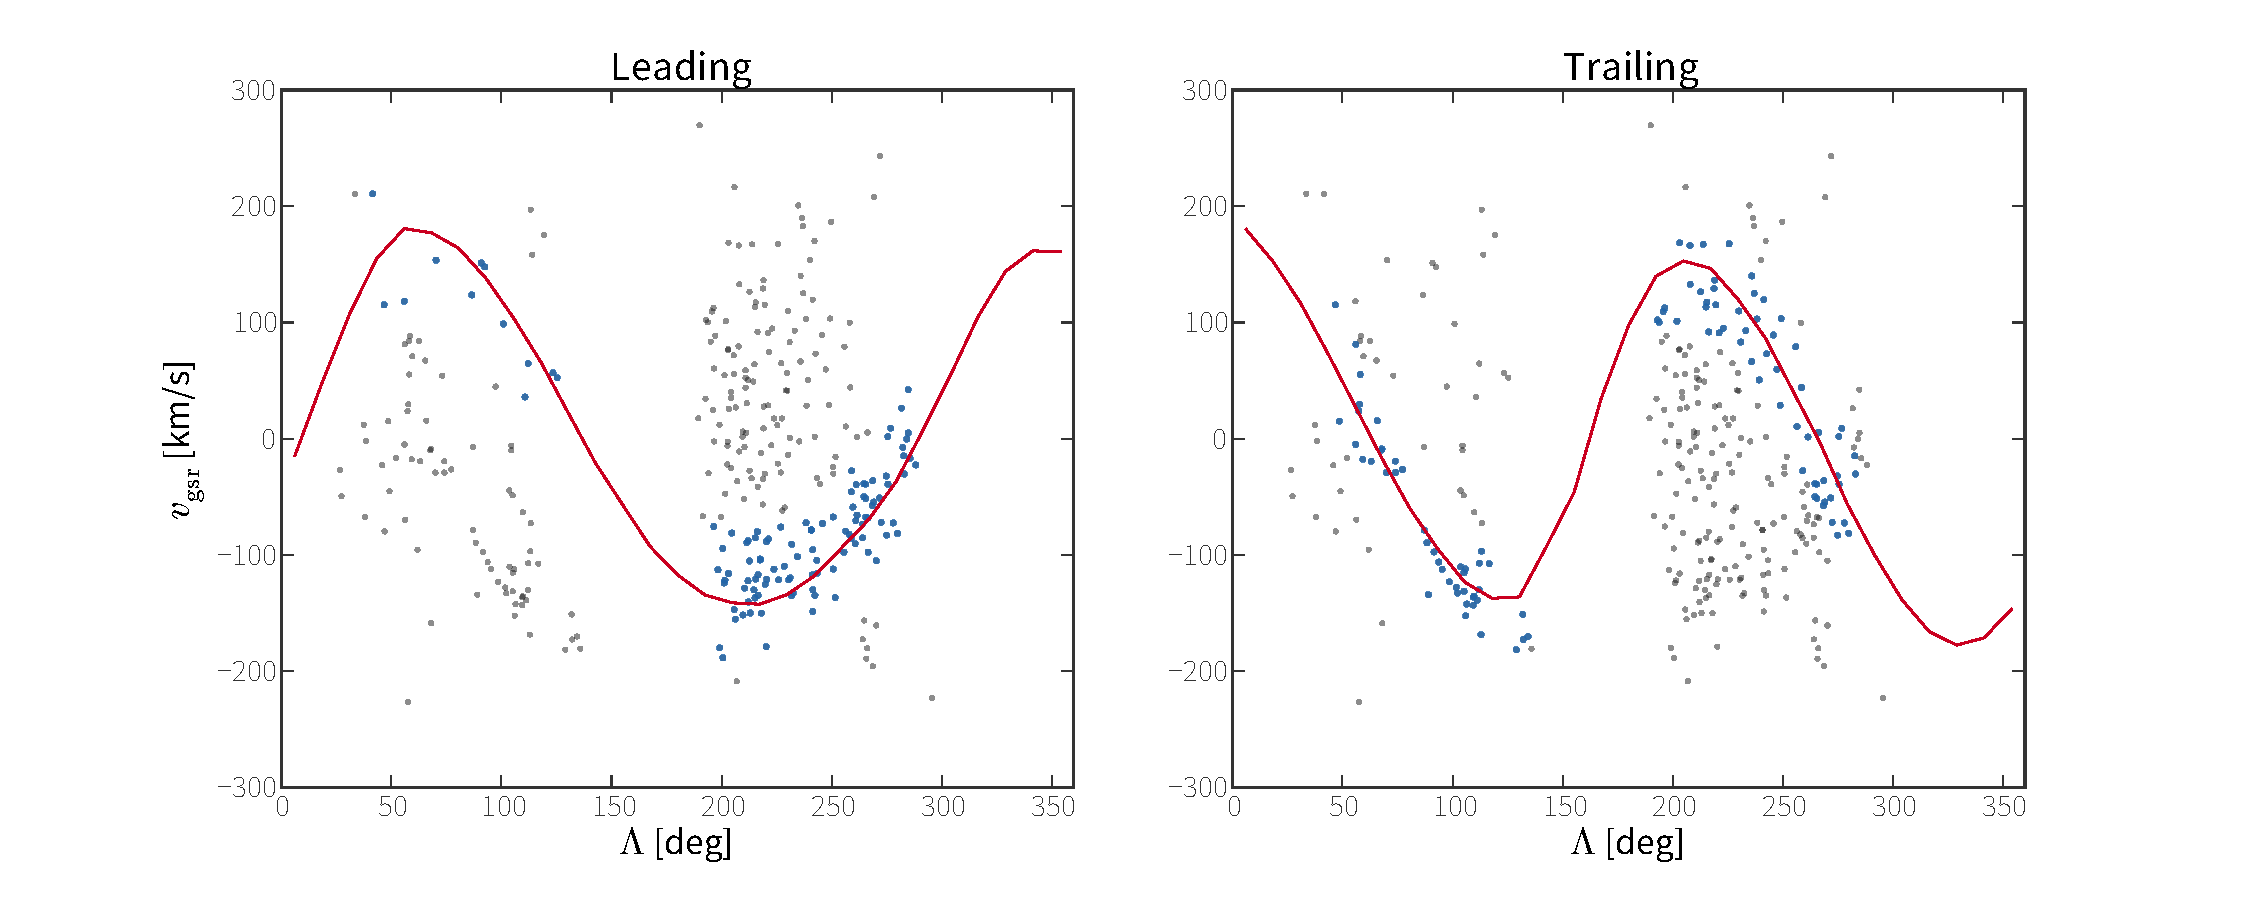
\includegraphics[width=\textwidth]{css_selection_from_vgsr.pdf}
\caption{ CSS RRLs selected to be within $\pm$3-$\sigma$ from the median LM10 radial velocity in each bin from fig.~\ref{fig:lm10_vgsr}. }\label{fig:css_vgsr}
\end{center}
\end{figure}

\begin{figure}
\begin{center}
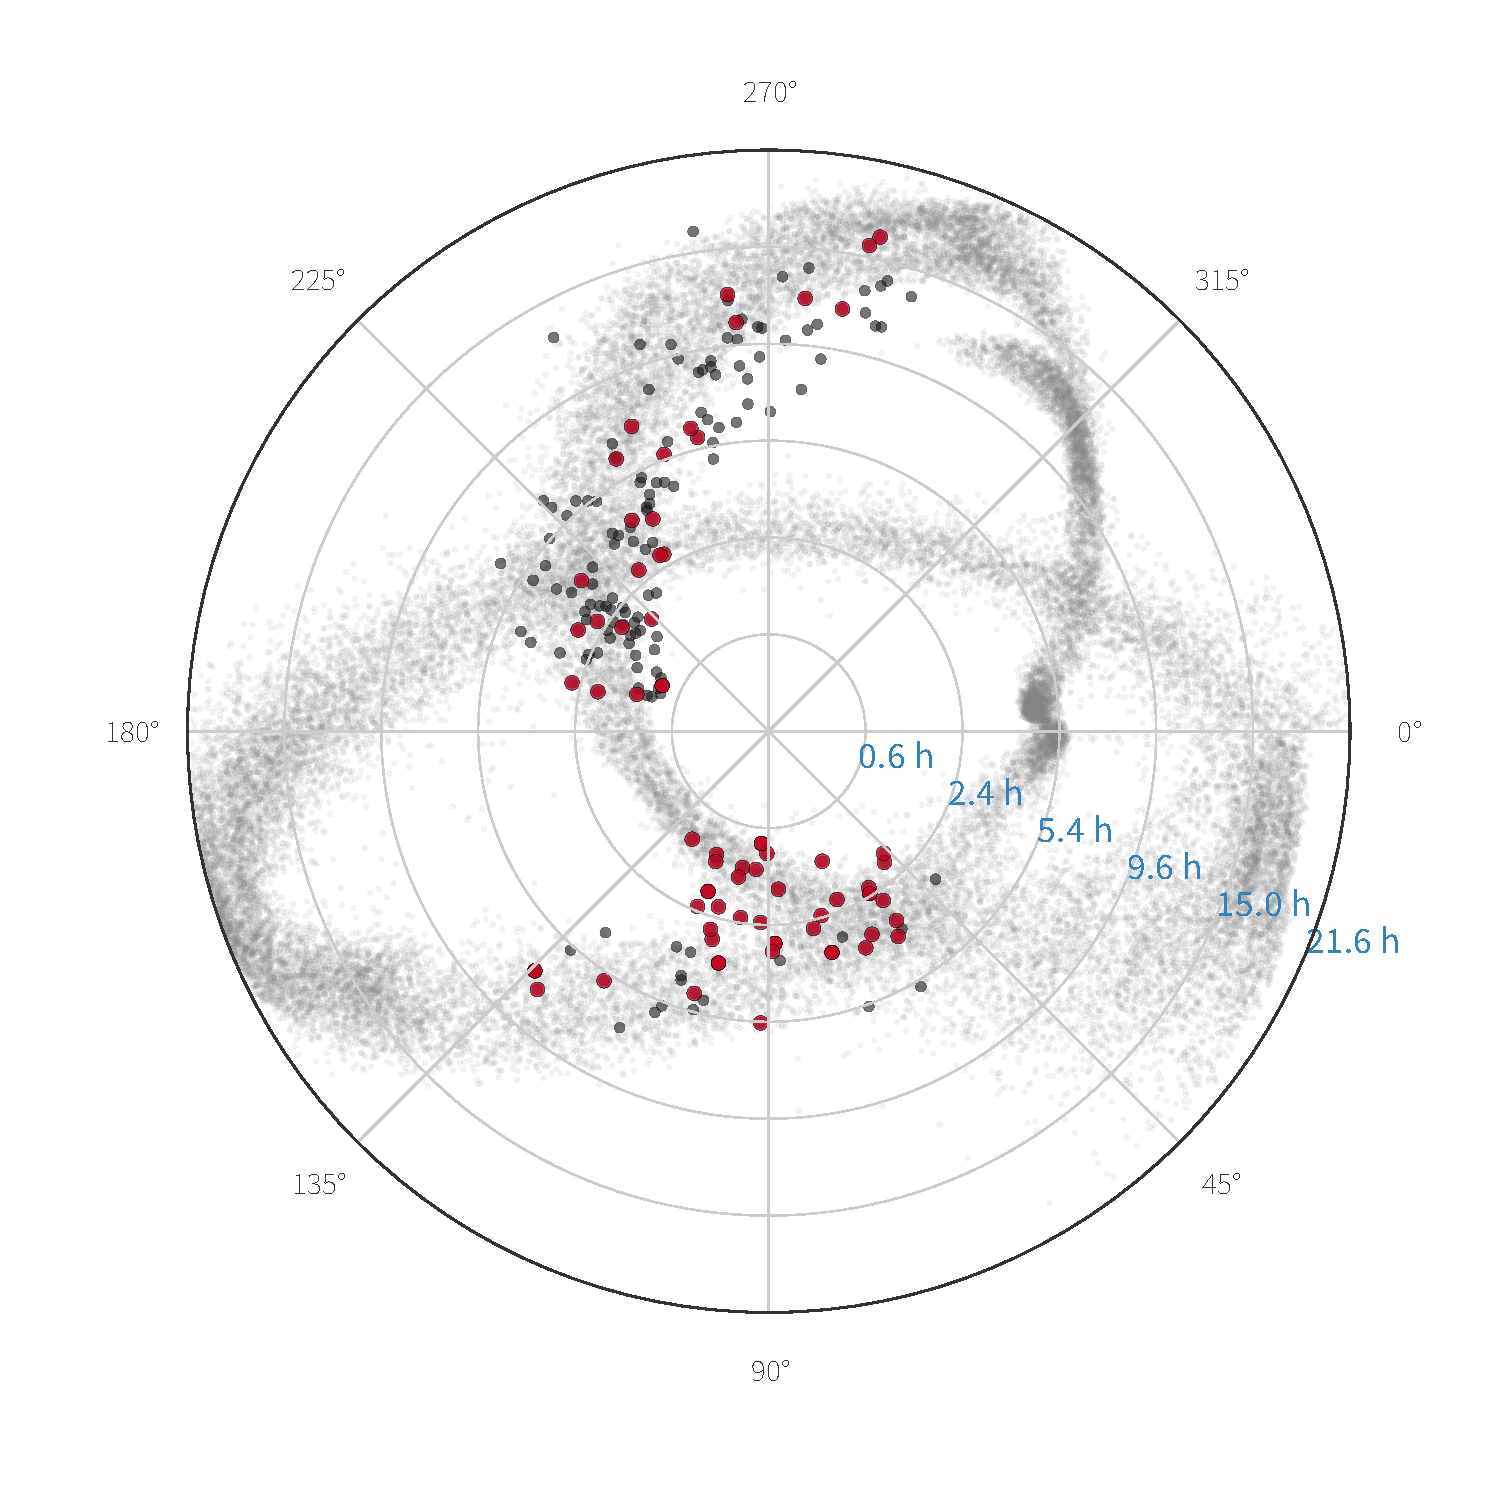
\includegraphics[width=\textwidth]{final_sample.pdf}
\caption{ Final sample of CSS RRLs selected to be observed with Spitzer (red) and other RRLs that meet the criteria, but are unable to observe due to time constraints. Concentric circles with labels show required total integration time (over 12 visits) for a typical RR Lyrae at that distance. }\label{fig:final_sample}
\end{center}
\end{figure}

\end{document}
